\section{Entschlüsseln}
\subsection{Grundlagen}

Um einen chiffrierten Text zu entschlüsseln beginnt man grundlegend mit der Kryptoanalyse. 
Die Kryptoanalyse hat das Ziel, Informationen über den Inhalt eines chiffrierten
Textes auch ohne Kenntnis des Schlüssels zu erhalten. Es werden verschiedene
Angriffsszenarien auf ein Kryptosystem unterschieden. Da lediglich der
chiffrierte Text bekannt war, wurde Ciphertext-Only gewählt. Es wurde mit der
Häufigkeitsanalyse begonnen.

\subsubsection{Häufigkeitsanalyse}

\begin{figure}
 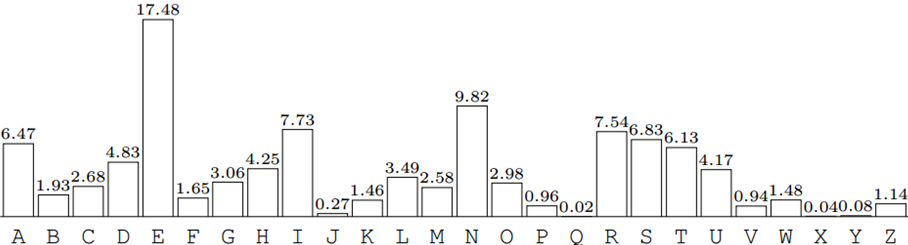
\includegraphics[width=\textwidth,keepaspectratio=true]{Images/buchstabenhaeufigkeiten_de}
 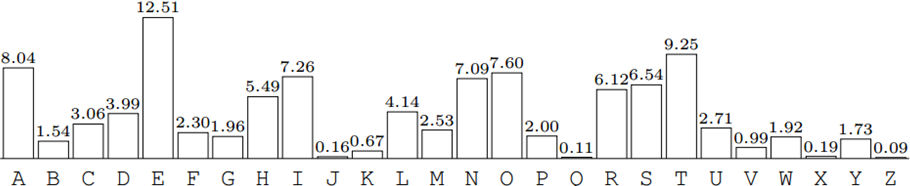
\includegraphics[width=\textwidth,keepaspectratio=true]{Images/buchstabenhaeufigkeiten_en}
 \caption{Häufigkeitsverteilung von Buchstaben im Deutschen (oben) und Englischen (unten) \cite[kap2.pdf, s. 30]{Koebler}}
 \label{fig:buchstabenhaeufigkeiten}
\end{figure}

In jeder Sprache kommen die einzelnen Buchstaben in einem ausreichend langen,
natürlichen Text in einer für die Sprache charakteristischen Häufigkeit vor
(siehe \cref{fig:buchstabenhaeufigkeiten}). Im Deutschen ist der am
häufigsten vorkommende Buchstabe das E mit einer Häufigkeit von etwa 17\,\%,
gefolgt vom N mit etwa 10\,\%.

\subsubsection{Caesar Chiffre}

Der Name Caesar-Chiffre stammt von dem gleichnamigen Feldherren Gaius Julius
Caesar (100 v. Chr. – 44 v. Chr.). Caesar benutzte diese sehr einfache Form der
Verschlüsselung, um militärische Nachrichten zu chiffrieren.  Es kann ein
beliebiges Alphabet verwendet werden. Die klassische Version benutzt die
Großbuchstaben A-Z. Das Alphabet wird zweimal, untereinander aufgeschrieben.
Nun wird das untere Alphabet um eine beliebige Anzahl Stellen verschoben. Diese
Anzahl von Stellen ist der Schlüsselwert der Chiffre. Eine Verschiebung um 3
nach links, also mit dem Schlüssel 3, ergibt folgende Ansicht:

\begin{lstlisting}
ABCDEFGHIJKLMNOPQRSTUVWXYZ
DEFGHIJKLMNOPQRSTUVWXYZABC

ZNAQRYFGHGRA  -> WKXNOVCDEDOX
\end{lstlisting}
